\subsection{Udledning af frekvens og positionsfunktion for harmonisk bevægelse}

Antag nu at Hookes lov gælder og at bevægelsen udelukkende foregår i y-aksens retning. Newton II giver da 

\bigskip

\begin{center}
$F_x = -k \cdot x = m \cdot a_x = m \cdot x'' \rightarrow a_x = -\dfrac{k}{m} \cdot x$
\end{center}

\bigskip

Hvis massen, m, af objektet der er fæstnet til fjederen er konstant er størrelsen $\dfrac{k}{m}$ bare en konstant og da er $a_x \propto x$ til et hvert tidspunkt. Ud fra dette kan vi se at accelerationen er størst når x har opnået sin højeste positive værdi, kald denne størrelse $x_{max}$. Ydermere vil accelerationen være lig 0 når objketet passerer sit hvilepunkt, da x er lig 0 i det punkt.
\pagebreak

Der bruges nu princippet om energibevarelse med den potentielle energi af systemet givet ved $V=\dfrac{1}{2} \cdot k \cdot x^2$, ligesom i afsnit 2.1.2 om Hookes lov, og den kinetiske energi af systemet givet ved $E_kin = \dfrac{1}{2} \cdot m \cdot v^2$.

\bigskip

\begin{center}
$E_{system}=\dfrac{1}{2} \cdot m \cdot v^2 + \dfrac{1}{2} \cdot k \cdot x^2 = konstant$
\end{center}

\begin{figure}[ht!]
  \centering
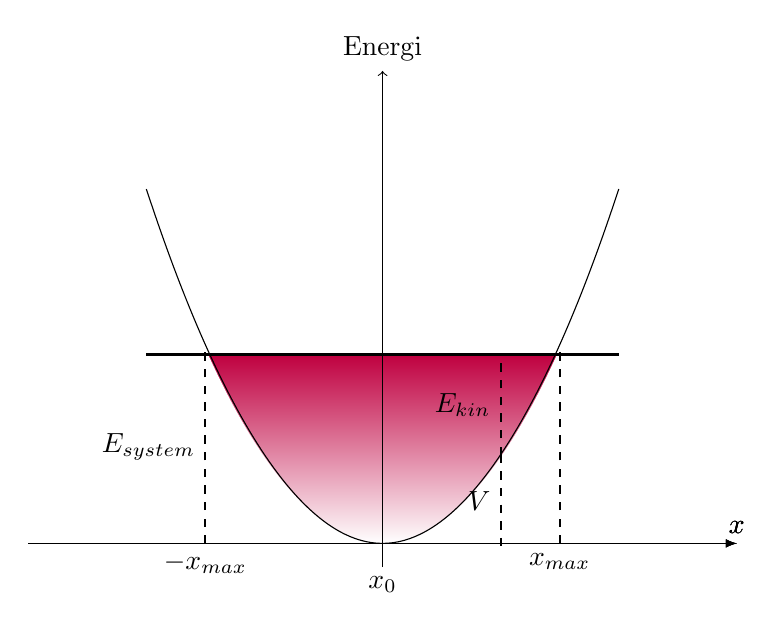
\begin{tikzpicture}[scale=1.5]
\shade[top color=purple,bottom color=white] (-1.49,0) rectangle (1.49,1.6);

\shade[top color=white,bottom color=white!50] 
      (0,0) parabola (1.5,1.65) |- (0,0);
\shade[top color=white,bottom color=white!50] 
      (0,0) parabola (-1.5,1.65) |- (0,0);      

  \draw[-latex] (-3,0) -- (3,0) node[above] {$x$};
  \draw[->] (0,-0.2) -- (0,4) node[above] {Energi};

  \draw (0,0) parabola bend (0,0) (2,3) node[below right] { };
  
  \draw (0,0) parabola bend (0,0) (-2,3) node[below right] { };
  
  \node[above] at (0,-0.5) {$x_0$};
  \draw[-latex] (-3,0) -- (3,0) node[above] {$x$};
	\draw[thick, dashed] (1,0.75) -- (1,1.6) node [midway, left] {$E_{kin}$};
	
	\draw[-latex] (-3,0) -- (3,0) node[above] {$x$};
	\draw[thick, dashed] (1,0.75) -- (1,-0.03) node [midway, left] {$V$};
	
	\draw[thick, dashed] (-1.5,0) -- (-1.5,1.63) node [midway, left] {$E_{system}$};
	
	\node[below] at (-1.5,0) {$-x_{max}$};
	
\draw[thick, dashed] (1.5,0) -- (1.5,1.63) node [midway, left] { };	

\node[below] at (1.5,0) {$x_{max}$};

\draw[very thick] (-2,1.6) -- (2,1.6) node [midway, left] { };

\end{tikzpicture}
\caption{$E_{system} $ for oscilerende bevægelse} \end{figure}

\bigskip

Den totale energi $E_{system}$ er ydermere også relateret til amplituden af $x_{max}$ sådan at når objektet når sin maksimale flytning $\pm x_{max}$ vil objektet stoppe og vende om. I dette punkt hastigheden $v = 0$ og objektet har altså ikke nogen kinetisk energi. I dette punkt er $E_{system } = \dfrac{1}{2} \cdot k \cdot x^2$. Derfor må det gælde at

\bigskip
\begin{center}
$E_{system}=\dfrac{1}{2} \cdot m \cdot v^2 + \dfrac{1}{2} \cdot k \cdot x^2 = \dfrac{1}{2} \cdot k \cdot (x_{max})^2$
\end{center}
\bigskip

eller 

\bigskip
\begin{center}
$\dfrac{1}{2} \cdot m \cdot v^2 + \dfrac{1}{2} \cdot k \cdot x^2 = \dfrac{1}{2} \cdot k \cdot (x_{max})^2 \rightarrow m \cdot v^2 = k \cdot (x_{max})^2 - k \cdot x^2 = k \cdot ((x_{max})^2 - x^2)$

$\rightarrow v^2 = \dfrac{k}{m} \cdot ((x_{max})^2 - x^2) \rightarrow v = \pm \sqrt[2]{\dfrac{k}{m}} \cdot \sqrt[2]{(x_{max})^2-x^2}$
\end{center}
\bigskip

Med forbehold for fortegnet kan vi bruge denne relation til at bestemme hastigheden af objektet til en hver position x. Vigtigheden af det fundne udtryk $v = \pm \sqrt[2]{\dfrac{k}{m}} \cdot \sqrt[2]{(x_{max})^2-x^2}$ gør sig tydligt på Figur (MANGLER) hvor energien er plottet op ad 2. aksen og udstrækningen fra hvilepositionen $x_0$ ad 1. aksen. Kurven repræsenterer den potentielle energi givet ved forskriften $V=\dfrac{1}{2} \cdot k \dot x^2$ og dette er en parabel. I højden E er der en tyk sort streg, som repræsenterer den energibevarelse der er for systemet, da den skærer parablen i netop $-x_{max}$ og $x_{max}$ som er yderpositionerne for bevægelsen. Til en vilkårlig udstrækning af fjederen kan vi også bestemme den kinetiske energi som længden af den linje, der går fra den horisontale linje ned til parablen ved netop den x-værdi. Dér hvor den kinetiske energi er størst og altså farten er størst er ved hvilepositionen $x_0$. Det gælder altså at

\bigskip
\begin{center}
$\dfrac{1}{2} \cdot m \cdot (v_{max})^2 = E_{system}$ eller $v_{max} = \sqrt[2]{\dfrac{2 \cdot E_{system}}{m}}$
\end{center}
\bigskip

Men da det netop gjorde sig gældende at den maksimale potentielle og kinetiske energi begge er lig systemets energi $E_{system}$, og derfor også til hinanden, kan vi relatere $v_{max}$ til $x_{max}$.

\begin{center}
\begin{equation}
E_{system} = \dfrac{1}{2} \cdot k \cdot (x_{max})^2 = \dfrac{1}{2} \cdot m \cdot (v_{max})^2 \rightarrow v_{max} = \sqrt[2]{\dfrac{k}{m}} \cdot x_{max}
\end{equation}
\end{center}

I ligning (MANGLER) fandt vi udtrykket $v = \pm \sqrt[2]{\dfrac{k}{m}} \cdot \sqrt[2]{(x_{max})^2-x^2}$. Dette beskrev hastigheden til en udstrækning x. Vi ser os ikke tilfredse med en hastighedsfunktion. Vi vil også have stedsfunktionen. Denne findes ved at skrive den fundne ligning op som 

\begin{center}
\begin{equation}
\dfrac{dx}{dt} = v = \pm \sqrt[2]{\dfrac{k}{m}} \cdot \sqrt[2]{(x_{max})^2-x^2}
\end{equation}
\end{center}

Men da kan ligningen integreres og løses for x, hvilket giver

\begin{center}
\begin{equation}
x = x_{max} \cdot sin(\sqrt[2]{\dfrac{k}{m}} \cdot t + C)
\end{equation}
\end{center}
\bigskip
Hvor C er en konstant. Notér at sinus er en periodisk funktion og at positionen af x altså også er en periodisk funktion af tiden, som vi forventede. Perioden for bevægelsen, T, er den tid det tager for systemet at lave en oscilation. Da sinusfunktionen gentager sig selv, hver eneste gang vi øger udtrykket inden i parantesen $sin(\sqrt[2]{\dfrac{k}{m}} \cdot t + C$ må det altså gælde, hvis vi starten til t = 0 at en oscilation må tage

\begin{center}
\begin{equation}
\sqrt[2]{\dfrac{k}{m}} \cdot T = 2 \pi \rightarrow T = 2 \pi \sqrt[2]{\dfrac{m}{k}}
\end{equation}
\end{center}

Hvilket hvis $f = \dfrac{1}{T}$ giver

\begin{center}
\begin{equation}
f = \dfrac{1}{T} = \dfrac{1}{2 \pi} \cdot \sqrt[2]{\dfrac{k}{m}}
\end{equation}
\end{center}

Hvilket er et vigtigt resultat, som vi vil bruge til at bestemme bølgetal for funktionelle grupper i IR-spektroskopien. 
\pagebreak